% Please make sure you insert your
% data according to the instructions in PoSauthmanual.pdf
\documentclass[a4paper,11pt]{article}
\usepackage{pos}
\usepackage{sidecap}    
\sidecaptionvpos{figure}{m}    
\sidecaptionvpos{table}{m}    
\usepackage{cleveref}    
\usepackage{enumitem}
\setitemize{itemsep=0pt,parsep=1pt,topsep=1pt,itemindent=0pt,leftmargin=9pt}    
\setenumerate{itemsep=0pt,parsep=1pt,topsep=1pt,itemindent=10pt,leftmargin=9pt}    
\usepackage{natbib}    
\setlength{\bibsep}{2pt}    
\setlength{\parindent}{0pt}    

\usepackage{listings}

\definecolor{codegreen}{rgb}{0,0.6,0}
\definecolor{codegray}{rgb}{0.5,0.5,0.5}
\definecolor{codepurple}{rgb}{0.58,0,0.82}
\definecolor{backcolour}{rgb}{0.95,0.95,0.92}

\lstdefinestyle{mystyle}{
    backgroundcolor=\color{backcolour},   
    commentstyle=\color{codegreen},
    keywordstyle=\color{magenta},
    numberstyle=\tiny\color{codegray},
    stringstyle=\color{codepurple},
    basicstyle=\ttfamily\tiny,
    breakatwhitespace=false,
    breaklines=true, 
    captionpos=b,
    keepspaces=true,
    numbers=left,
    numbersep=5pt,
    showspaces=false,
    showstringspaces=false,
    showtabs=false,
    tabsize=2
}

\lstset{style=mystyle}

\usepackage{algorithm}
\usepackage{algorithmicx}
\usepackage{algpseudocode}

\usepackage[font={small,it},labelfont=bf,tableposition=top]{caption}

\title{Status of the ETMC ensemble generation effort}
%% \ShortTitle{Short Title for header}

\author{Constantia Alexandrou$^{a,b}$}
\author{Simone Bacchio$^b$}
\author{Jacob Finkenrath$^c$}
\author{Roberto Frezzotti$^d$}
\author*{Marco Garofalo$^e$}
\author*{Bartosz Kostrzewa$^e$}
\author{Giannis Koutsou$^b$}
\author{Simone Romiti$^f$}
\author{Aniket Sen$^e$}
\author{Carsten Urbach$^e$}
\author{Urs Wenger$^f$}

\affiliation[a]{Department of Physics, University of Cyprus, 20536 Nicosia, Cyprus}
\affiliation[b]{Computation-based Science and Technology Research Center, The Cyprus Institute, 2121 Nicosia, Cyprus}
\affiliation[c]{Theoretical Physics Department, CERN 1211 Geneva 23, Switzerland}
\affiliation[d]{Dipartimento di Fisica and INFN, Universit{\`a} di Roma ``Tor Vergata'', I-00133
\affiliation[e]{Helmholtz-Institut für Strahlen und Kernphysik (Theory), Rheinische Friedrich-Wilhelms-Universität Bonn, Nussallee 14-16, 53115 Bonn, Germany}
\affiliation[f]{Institute for Theoretical Physics, Albert Einstein Center for Fundamental Physics, University of Bern, CH-3012 Bern, Switzerland}

\emailAdd{alexandrou.constantia@ucy.ac.cy}
\emailAdd{s.bacchio@cyi.ac.cy}
\emailAdd{j.finkenrath@cern.ch}
\emailAdd{roberto.frezzotti@roma2.infn.it}
\emailAdd{garofalo@hiskp.uni-bonn.de}
\emailAdd{kostrzewa@hiskp.uni-bonn.de}
\emailAdd{g.koutsou@cyi.ac.cy}
\emailAdd{simone.romiti@unibe.ch}
\emailAdd{sen@hiskp.uni-bonn.de}
\emailAdd{urbach@hiskp.uni-bonn.de}
\emailAdd{urs.wenger@unibe.ch}

\abstract{We present a status report on the ETMC ensemble generation effort toward controlled continuum and infinite volume extrapolations for a variety of physical observables through simulations employing $N_f = 2+1+1$ Wilson clover twisted mass fermions at physical quark masses using five lattice spacings.
We further given an update on the status of the tmLQCD software suite.
Through extensions of the QUDA lattice QCD library and a corresponding interface in tmLQCD, we are able to offload a significant portion of our HMC to GPUs, enabling efficient simulations on the current generation of heterogeneous machines.
\vspace{2cm}
\begin{center}
  
\includegraphics[width=0.35\linewidth]{plots/Logo_ETMC_RGB}
\end{center}
}

\FullConference{The 41st International Symposium on Lattice Field Theory (LATTICE2024)\\
 28 July - 3 August 2024\\
Liverpool, UK\\}

%% \tableofcontents

\begin{document}
\maketitle


\section{Introduction}

\begin{figure}
  \includegraphics[width=0.5\linewidth,page=2]{plots/quda_speedup}
  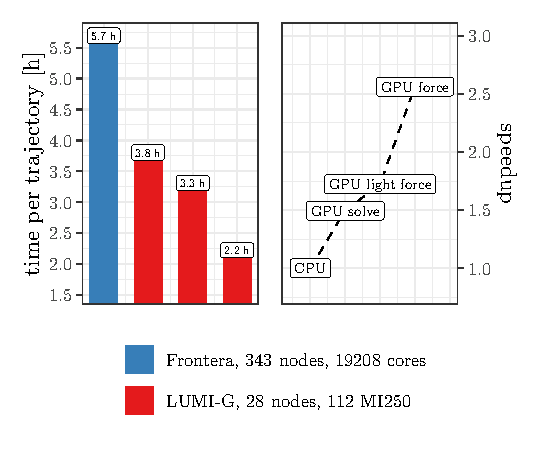
\includegraphics[width=0.5\linewidth,page=1]{plots/quda_speedup}
  \caption{\textbf{Left:} Time per $\tau=1.0$ trajectory of tmLQCD + QUDA (green) for a $64^3 \cdot 128$ ensemble at the physical point compared to the machine it was originally generated on (purple) using tmLQCD + DD-$\alpha$AMG~\cite{Alexandrou:2016izb}. The speedups demonstrate the effect of increasing levels of QUDA offloading. \textbf{Right:} The same kind of comparison between tmLQCD + QUDA and tmLQCD + DD-$\alpha$AMG + QPhiX~\cite{QPhiX,Schrock:2015gik,QPhiX-github} running a $112^3 \cdot 224$ ensemble at the physical point on LUMI-G and Frontera, respectively.}
  \label{fig:quda_speedup}
\end{figure}

\section{Acknowledgements}
{
\small
We would like to thank the QUDA developers for their tremendous work as well as the many pleasant and productive interactions during this and previous efforts. 
We thank the ETMC for the most enjoyable collaboration. 
For part of this work. S.B. and J.F. were supported by the H2020 project PRACE 6-IP (grant agreement No. 82376) and the EuroCC project (grant agreement No. 951740).
This project was funded by the Deutsche Forschungsgemeinschaft (DFG, German Research Foundation) as part of the CRC 1639 NuMeriQS – project no. 511713970. 
This work was supported by the Deutsche Forschungsgemeinschaft (DFG, German Research Foundation) and the NSFC through the funds provided to the Sino-German Collaborative Research Center CRC 110 “Symmetries and the Emergence of Structure in QCD” (DFG Project-ID 196253076 - TRR 110, NSFC Grant No. 12070131001).
We acknowledge support by the European Joint Doctorate program STIMULATE grant agreement No. 765048.
We acknowledge support from projects NextQCD (EXCELLENCE/0918/0129) and "3D-Nucleon" (EXCELLENCE/0421/0043), co-funded by the European Regional Development Fund and the Republic of Cyprus through the Research and Innovation Foundation. 
We further acknowledge: The Gauss Centre for Supercomputing e.V. for funding this project through computing time on the GCS supercomputers SuperMUC and SuperMUC-NG at Leibniz Supercomputing Center as well as JUWELS Booster~\cite{JUWELS,BOOSTER} at the Jülich Supercomputing Centre.
PRACE for awarding access to HAWK at HLRS within the project with Id Acid 4886. 
The Swiss National Supercomputing Centre (CSCS) and the EuroHPC Joint Undertaking for awarding access to the LUMI supercomputer, owned by the EuroHPC JU, hosted by CSC and the LUMI consortium through the Chronos programme under project IDs CH17-CSCS-CYP and CH21-CSCS-UNIBE as well as EuroHPC under project ID EHPC-REG-2021R0095.
The Texas Advanced Computing Center (TACC) at The University of Texas at Austin for providing HPC resources on Frontera~\cite{FRONTERA} (Project ID PHY21001).
The EuroHPC Joint Undertaking for awarding access to the Luxembourg national supercomputer MeluXina.
The University of Bonn for access to the Bender and Marvin clusters as well as support by the HRZ-HPC team.
}

\bibliographystyle{JHEP}
{\footnotesize
\bibliography{bibliography}
}

\end{document}
